\documentclass{beamercours}

\title{Cours TalENS 2023-2024}
\subtitle{Dérivée, Volume, Aire, Périmètre}
\date{chaipakan}

\begin{document}
\maketitle

    \section{Rappels Mathématiques}
        \subsection{Dérivation}
            \begin{frame}{Dérivée par rapport à une variable}
                \begin{definition}
                    Si $f$ est dérivable, $f^{'}(x) = \lim\limits_{\mathrm{d}x \rightarrow 0} \frac{f(x + \mathrm{d}x) - f(x)}{\mathrm{d}x}$. $f'(x)$ est la pente de la tangente à la courbe de $f$ en $x$.
                \end{definition}
                Toutes les fonctions que nous allons étudier seront dérivables, et même souvent rationnelles.
                Règles de dérivation usuelles : 
                \begin{itemize}
                    \item $\forall n \in \mathbb{Z},  \deriv{x}{x^{n}} = nx^{n-1}$
                    \item $\deriv{x}{\ln{(x)}} = \frac{1}{x}$
                    \item $\deriv{x}{f}g = \deriv{x}{f}g + f\deriv{x}{g} $
                \end{itemize}
            \end{frame}
            
            \begin{frame}{Règle de la chaîne - Changement de Variable}
                \begin{theorem}[Règle de la Chaîne]
                    Soit $f$ dérivable, $g$ dérivable : $(f(g(v))) = g'(v) \times f^{'}(g(v))$.
                \end{theorem}
                \begin{definition}[Changement de Variable]
                    On appelle poser dans $f$ le changement de $u = g(v)$ le fait d'écrire : $f(u) = f(g(v))$. On a alors : $\deriv{u}{f(u)} = \deriv{u}{v}\deriv{v}{f(g(v))}$
                \end{definition}
                Exemples : Poser le changement de variable $x = \exp y$ pour calculer la dérivée de $\deriv{x}{\ln(x)}$. 
            \end{frame}

        \subsection{Polygones Réguliers et Solides de Platon}
            \begin{frame}{Polygones Réguliers : Aire et Périmètre}
                Un $n$-gone régulier est un polygone (convexe) à $n$ côtés de même longueur $c$.\\
                On fait ici un abus de notation, en ne considérant que les polygones convexes pour parler des $n$-gones réguliers, pourquoi ?
                \begin{theorem}
                    En notant $\rho$ l'apothème du polygone (la distance du centre à un côté) :
                    \begin{itemize}
                        \item $P(n, c) = nc$
                        \item $A(n, c) = n\frac{c\rho}{2} = P(n, c)\frac{\rho}{2}$
                    \end{itemize}
                \end{theorem}
            \end{frame}

            \begin{frame}
                \frametitle{Un catalogue des Solides de Platon}
                \begin{definition}
                    Les solides de Platon sont les polyèdres réguliers convexes, i.e. des solides dont les faces sont planes polygonales régulières, similaires et se rencontrent selon des segemnts appelés arêtes.
                \end{definition}
                \begin{center}
                    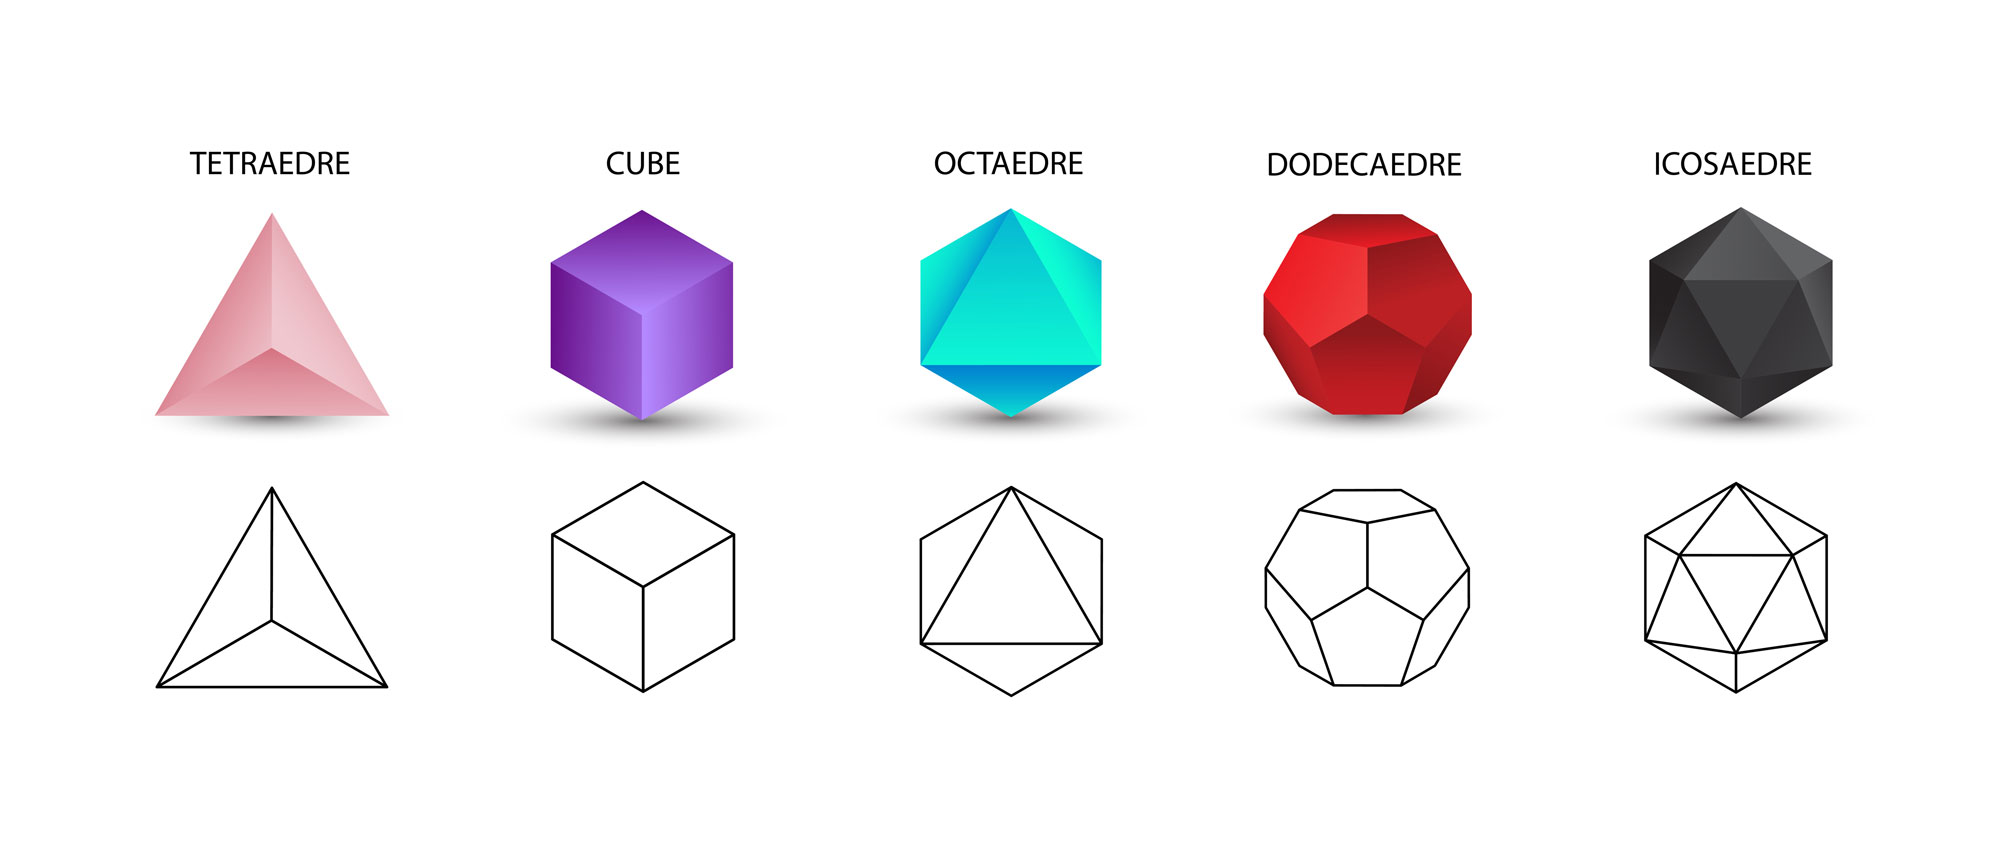
\includegraphics{solides-de-platon-02.jpg}    
                \end{center}
                
            \end{frame}

            \begin{frame}
                \frametitle{Exhaustivité}
                \begin{theorem}
                    Il y en a $5$ et seulement $5$: Le Tétraèdre (pyramide à ? faces), le cube (hexaèdre), l'octaèdre, le dodécaèdre, l'icosaèdre.
                \end{theorem}
                \begin{proof}
                    On a toujours : $S - A + F = 2$ et $pF = 2A = qS$, où $p$ est le nombre de côtés des faces, et $q$ le nombre de face se rejoignant à chaque sommet. 
                    On en déduit qu'on doit avoir : $\frac{1}{p} + \frac{1}{q} > \frac{1}{2}$. Mais comme $p, q \geq 3$, on n'a bien que $5$ possibilités qui sont autant de solides.\\
                \end{proof}                     
            \end{frame}

    \section{Constatations}
        \subsection{En Dimension 2 : Le Cercle}
            \begin{frame}{Rayon, Périmètre, Aire}

            \end{frame}

        \subsection{En Dimension 3 : La Sphère}

        \subsection{Presque Contre-Exemples}
            \begin{frame}{Le Carré}
                
            \end{frame}

            \begin{frame}{Le Triangle Equilatéral}
                
            \end{frame}

            \begin{frame}{Les $n$-gones Réguliers}
                
            \end{frame}

            \begin{frame}{Le Cube}
                
            \end{frame}

    \section{Généralisation}
        \subsection{L'Aire et le Volume en $d$ Dimensions}
            \begin{frame}{Un Espace en $d$ Dimensions ?}
            
            \end{frame}

            \begin{frame}{Un Solide en $d$ Dimensions}
                
            \end{frame}

            \begin{frame}{Aire et Volume d'un Solide en $d$ Dimensions}
                
            \end{frame}

        \subsection{Relation entre Volume et Aire en $d$ Dimensions pour un Solide}
            \begin{frame}{Le cas du Cube}
                
            \end{frame}


        \subsection{Et pour une forme quelconque ?}
            \begin{frame}{Famille Lisse de Formes Uni-Paramétrées}
                
            \end{frame}

            \begin{frame}{Famille Lisse de Formes $k$-Paramétrées}
                
            \end{frame}

\end{document}
